\section{Grundlagen} \label{grundlagen}

Dieses Kapitel ordnet die technischen und methodischen Grundlagen der Arbeit ein.

\subsection{Reverse Engineering, Re-Engineering und Forward Engineering}

Reverse Engineering, Re-Engineering und Forward Engineering bilden den klassischen begrifflichen Rahmen, in dem auch die vorliegende Arbeit verortet ist. Nach der Taxonomie von \textcite{chikofsky1990taxonomy} dient Reverse Engineering dazu, ein bestehendes System zu analysieren, seine Komponenten und Beziehungen zu identifizieren und daraus höherwertige Repräsentationen abzuleiten. Forward Engineering beschreibt dagegen den Weg von solchen Abstraktionen zurück in eine Implementierung. Re-Engineering verbindet beide Richtungen zu einem Erneuerungsprozess, bei dem ein bestehendes System verstanden, restrukturiert und in veränderter technischer Form neu umgesetzt wird \parencite{chikofsky1990taxonomy,raibulet2017mdre}.

Für gewachsene Softwaresysteme ist diese Unterscheidung besonders relevant, weil Migrationen in der Regel nicht als direkte Code-zu-Code-Übersetzung gelingen. Vielmehr muss der Bestandscode zunächst semantisch erschlossen werden, bevor fachliche Logik, Architekturentscheidungen und Randbedingungen in einer neuen technologischen Umgebung wieder implementiert werden können. Klassische Arbeiten zum Reverse Engineering objektorientierter Systeme betonen daher die Notwendigkeit, Codewissen schrittweise auf höhere Abstraktionsebenen zu heben \parencite{tonella2005reverseoo}.

\subsubsection{Horseshoe-Modell als Referenzrahmen}

Ein verbreitetes Denkmuster für diesen Ablauf ist das Horseshoe-Modell des Re-Engineering. Es veranschaulicht, dass der Weg von einem Quellsystem nicht direkt in eine Zielimplementierung führt, sondern über eine abstrahierte Zwischenebene verläuft, auf der Modelle, Architektursichten oder Spezifikationen explizit gemacht werden. Modellgetriebene Reverse-Engineering-Ansätze nutzen genau diese Zwischenebene als Brücke zwischen Analyse und Neuimplementierung \parencite{raibulet2017mdre}.

\begin{figure}[H]
\centering
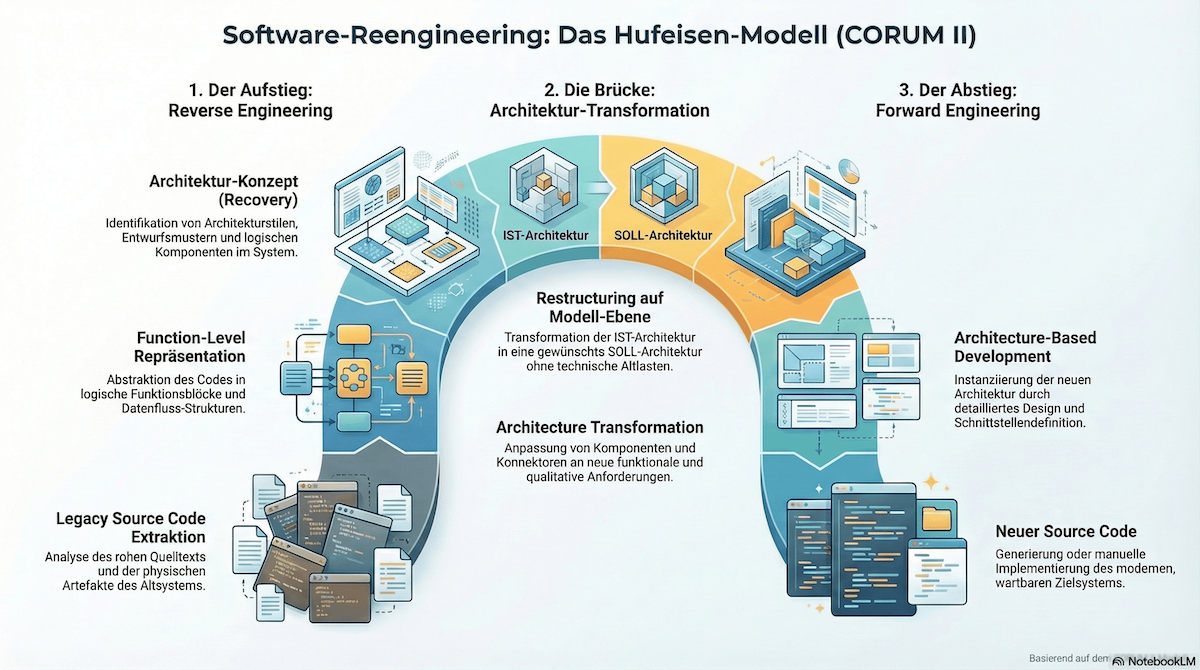
\includegraphics[width=0.9\textwidth,height=0.5025\textwidth,keepaspectratio]{abbildungen/horseshoe-modell.png}
\caption{Schematische Darstellung des Horseshoe-Modells für das Re-Engineering in Anlehnung an \textcite{raibulet2017mdre}.}
\label{fig:horseshoe-model}
\end{figure}

In der vorliegenden Arbeit wird diese Abstraktionsebene nicht primär durch formale Modelle, sondern durch textuelle technische Spezifikationen realisiert. Damit bleibt das Grundmuster des Re-Engineering erhalten, wird jedoch um einen spec-getriebenen und agentisch orchestrierten Verarbeitungsschritt erweitert.

\subsubsection{Agentenbasierte Code-Migration als Sonderfall des Re-Engineering}

Agentenbasierte Code-Migration beschreibt Migrationsprozesse, bei denen spezialisierte Software-Agenten einzelne Aufgaben des Reverse Engineering, der Wissensextraktion, der Spezifikation und der Code-Erzeugung übernehmen. In der vorliegenden Arbeit wird sie damit nicht als eigenständige Disziplin neben dem Re-Engineering verstanden, sondern als ein KI-gestützter Sonderfall dieses übergeordneten Erneuerungsprozesses. Gegenüber monolithischen Ansätzen verspricht diese Form der Aufgabenteilung eine bessere Nachvollziehbarkeit und klarere Verantwortlichkeiten. Einen aktuellen Überblick über Ansätze mit großen Sprachmodellen im Reverse Engineering geben \textcite{hu2025sokreverseengineering}. Erste Arbeiten behandeln dabei unter anderem generative KI für Re-Engineering-Szenarien in Software-Produktlinien, LLM-gestützte Werkzeugunterstützung im model-driven Reverse Engineering sowie die Ableitung von Sequenzdiagrammen aus Quellartefakten \parencite{acher2023splreengineering,boronat2025mdrellm,greiner2025sequencediagrams}.

Ein wesentlicher Schwierigkeitsfaktor der Migration liegt in technologischen Brüchen zwischen Quell- und Zielsystem. Unterschiede in Typisierung, Laufzeitmodell, Fehlerbehandlung oder Nebenläufigkeit erschweren eine rein syntaktische Übertragung und machen eine semantische Rekonstruktion der Fachlogik erforderlich. Werden große Sprachmodelle (Large Language Models, LLMs) in solchen Migrationsprozessen eingesetzt, entsteht zusätzlich die Herausforderung nicht-deterministischer Ausgaben. Halluzinationen und inkonsistente Ableitungen gefährden insbesondere bei umfangreichen Codebasen die Korrektheit der Ergebnisse. Deshalb müssen generierte Artefakte gegen belastbare Quellinformationen überprüft werden.

\subsection{Spec-Driven Development}

Spec-Driven Development verlagert den Schwerpunkt der Migration von der unmittelbaren Code-Erzeugung auf eine vorgelagerte Beschreibung der fachlichen und technischen Anforderungen. Die Spezifikation fungiert dabei als Zwischenartefakt, das sowohl der Analyse als auch der späteren Generierung als Referenz dient. Auf der Ebene aktueller KI-Werkzeuge beschreibt \textcite{boeckeler2025sdd} diesen Ansatz als Verschiebung von einem reinen ``Prompt-to-Code''-Muster hin zu einem Vorgehen, bei dem zunächst ein belastbares Spec-Artefakt erzeugt und anschließend als Anker für weitere Implementierungsschritte genutzt wird.

\begin{figure}[H]
\centering
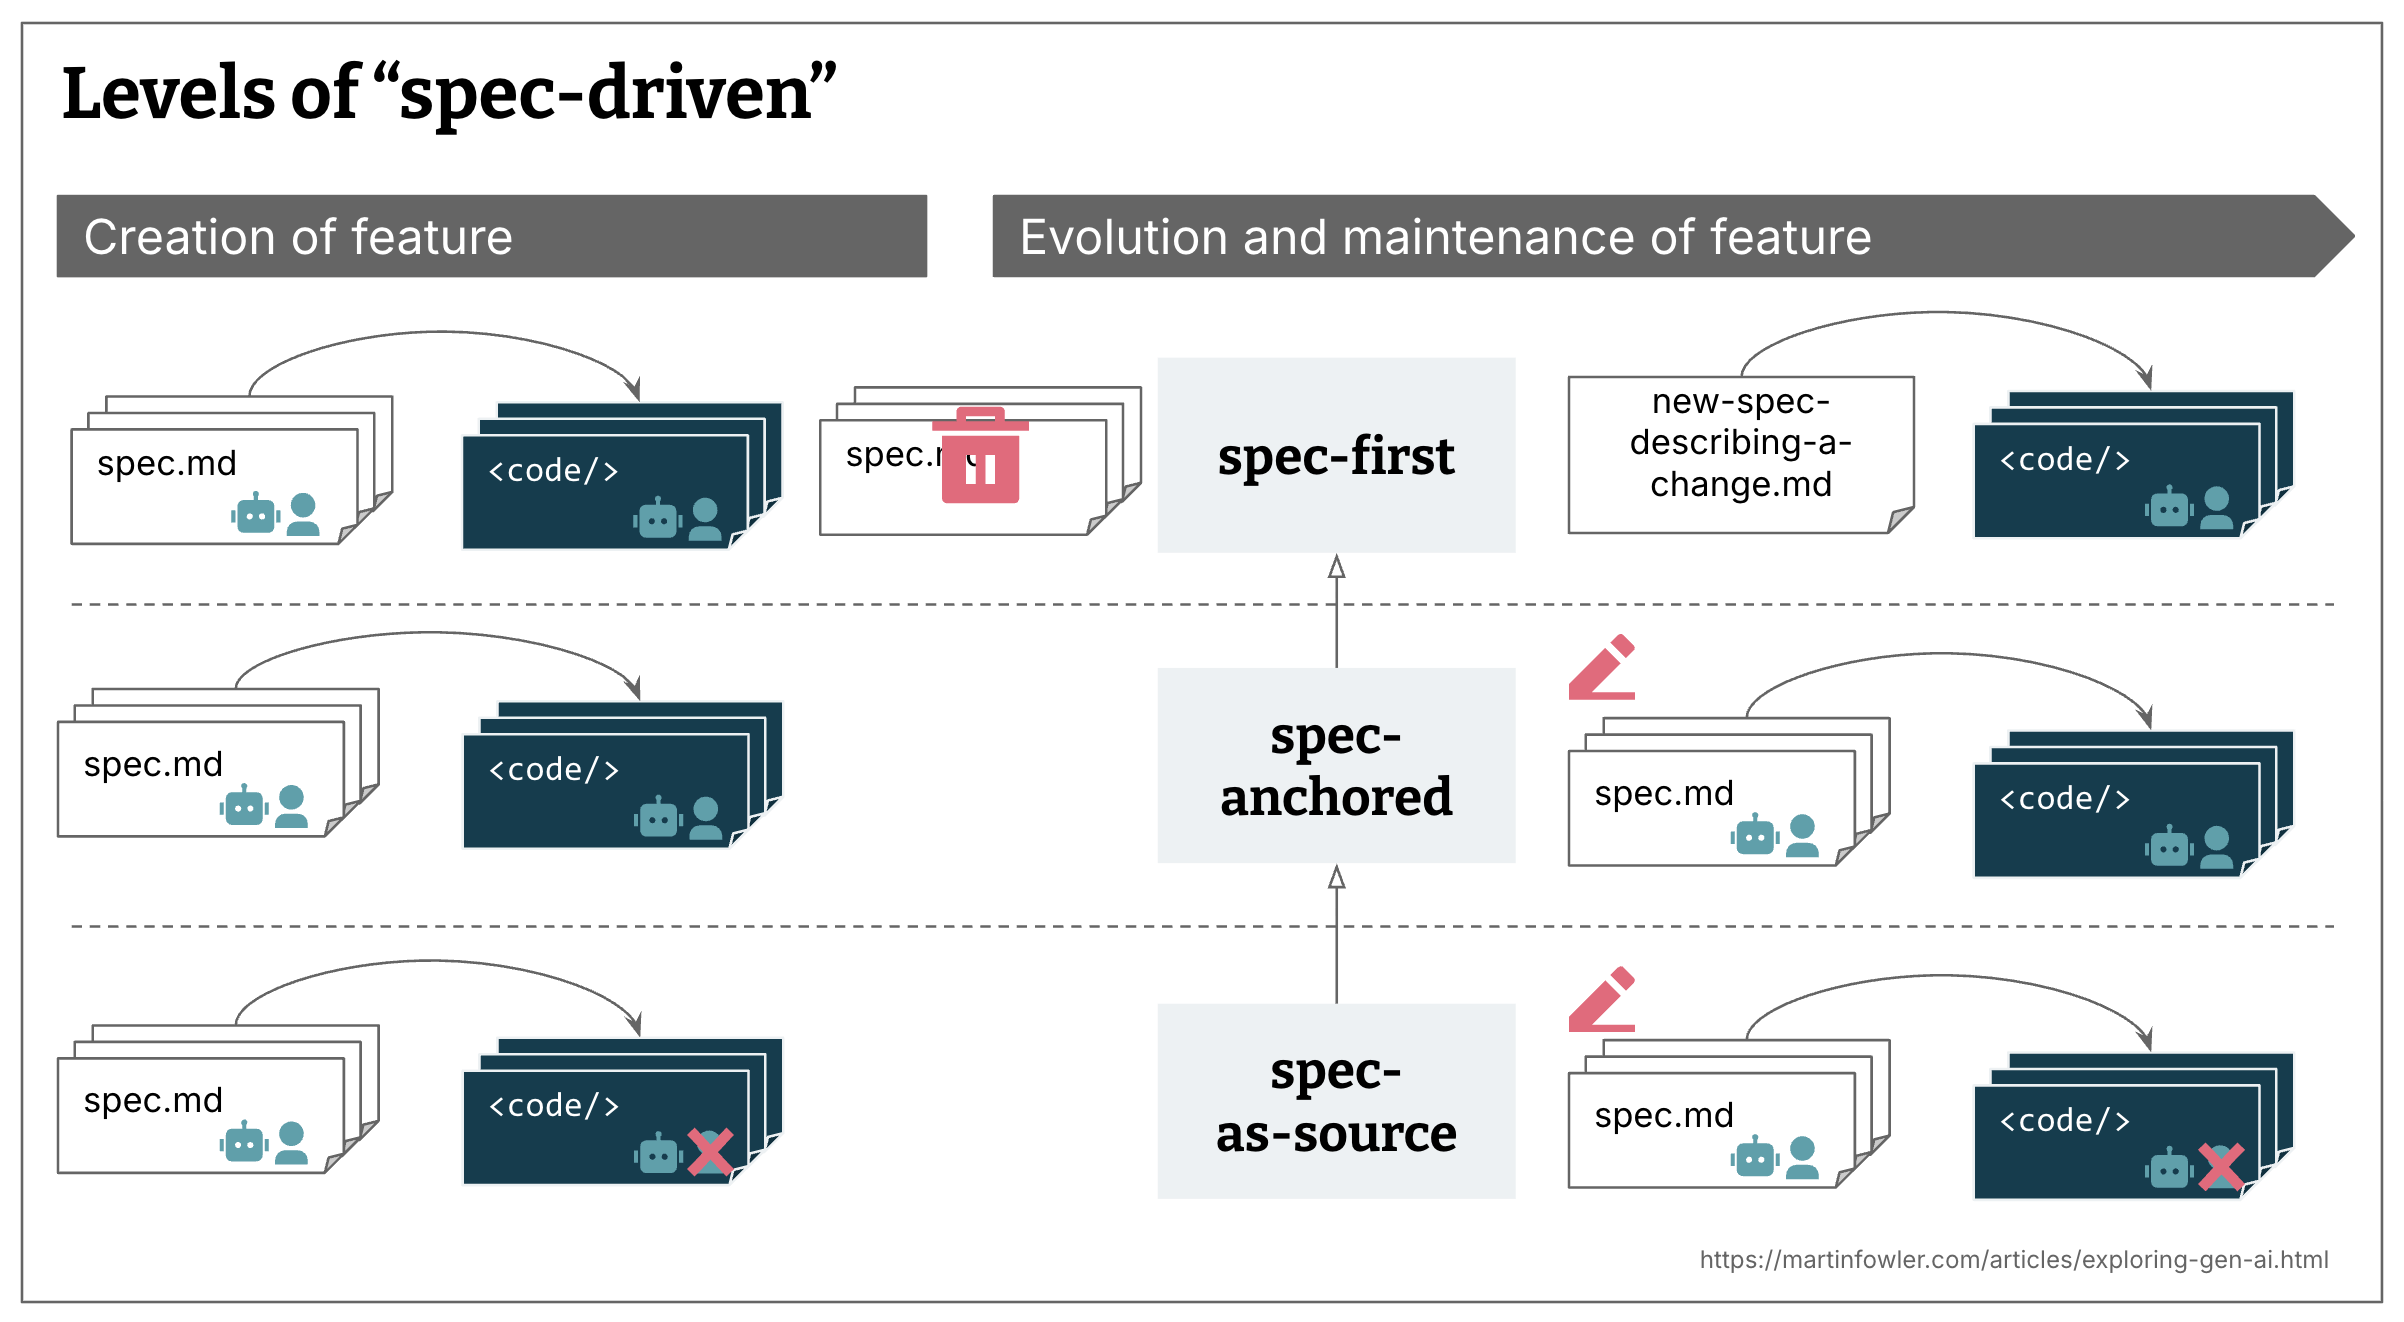
\includegraphics[width=0.9\textwidth,height=0.4948\textwidth,keepaspectratio]{abbildungen/fowler-sdd-levels.png}
\caption{Abbildung zu Ausprägungen und Reifegraden von Spec-Driven Development aus \textcite{boeckeler2025sdd}. Für die vorliegende Projektarbeit ist insbesondere die spec-first Ausprägung relevant, in der zunächst ein belastbares Spezifikationsartefakt erzeugt wird, bevor die eigentliche Implementierung beginnt.}
\label{fig:sdd-varianten}
\end{figure}

\subsubsection{Das Konzept „Specification First“ im Software-Reengineering}

Im Software-Reengineering bedeutet ``Specification First'', dass vorhandene Systemlogik zunächst rekonstruiert und in eine explizite technische Beschreibung überführt wird. Dadurch wird Wissen aus schwer zugänglichem Bestandscode in eine Form gebracht, die überprüfbar und transformierbar ist. Für die Überführung des vorhandenen Codes in Anforderungen ist dabei die Brücke zwischen Reverse Engineering und Requirements Engineering zentral \parencite{fahmi2007reverse}. Gleichzeitig lässt sich dieser Gedanke mit Fowlers Verständnis von Spezifikationen als präzisierenden Arbeitsartefakten verbinden: In ``Specification by Example'' argumentiert \textcite{fowler2004specificationbyexample}, dass Beispiele und konkretisierte Verhaltensbeschreibungen nicht bloß Dokumentation sind, sondern ein Mittel, um Anforderungen, erwartetes Verhalten und spätere Verifikation enger miteinander zu koppeln. Für die vorliegende Arbeit ist dieser Gedanke besonders relevant, weil die technische Spezifikation nicht nur beschreibend, sondern auch prüfbar und für nachgelagerte Agenten operationalisierbar sein soll.

\subsubsection{Vorteile der Abstraktion gegenüber direkter Code-Transpilierung}

Die Abstraktion über Spezifikationen bietet Vorteile gegenüber direkter Transpilierung, weil sie architektonische Intentionen, Fachlogik und Randbedingungen explizit macht. Damit sinkt das Risiko, dass ein Zielsystem zwar syntaktisch korrekt, aber konzeptionell fehlerhaft oder schwer wartbar entsteht. Aus Fowler-Perspektive lässt sich dies zusätzlich über die Idee domänenspezifischer Sprachen und semantischer Modelle begründen: Werden Anforderungen in eine fachlich lesbare, strukturierte Form überführt, entsteht ein robusteres Bindeglied zwischen Problemraum und technischer Umsetzung \parencite{fowler2010dsl}. Für den PoC der Projektarbeit wird keine vollwertige DSL entwickelt, wohl aber ein textuelles Spec-Artefakt mit ähnlicher Funktion: Es strukturiert Fachlogik, Schnittstellen und Randfälle so, dass spätere Generierungsschritte nicht ausschließlich auf impliziten Annahmen im Quellcode oder im Prompt beruhen.

Die empirische Untersuchung von \textcite{midolo2026promptguidelines} legt zudem nahe, dass explizite Angaben zu Ein- und Ausgabeformaten, Vor- und Nachbedingungen sowie Beispielen die Erfolgswahrscheinlichkeit in der nachgelagerten Codegenerierung deutlich erhöhen. Diese Beobachtung stützt den spec-getriebenen Fokus der vorliegenden Arbeit. Im Sinne von \textcite{boeckeler2025sdd} ist die Spezifikation damit nicht nur Dokumentation, sondern das zentrale Koordinationsartefakt zwischen Analyse, Verifikation und Generierung.

Im Kontext des Horseshoe-Modells passt für die vorliegende Projektarbeit vor allem eine spec-first Ausprägung. Zunächst wird die bestehende Funktionalität durch Analyse und Reverse Engineering in ein eigenständiges Spezifikationsartefakt überführt. Erst auf dieser Grundlage beginnt die eigentliche Entwicklung des Zielsystems. Die Spezifikation ist damit nicht nur begleitender Anker, sondern die verbindliche Übergabeschicht zwischen Rekonstruktion und Neuimplementierung. Gerade für einen PoC ist diese Reihenfolge sinnvoll, weil sie den Nutzen expliziter Spezifikation sichtbar macht, ohne bereits einen vollständig modell- oder DSL-basierten Generierungsansatz vorauszusetzen.

\subsection{Multi-Agenten-Systeme und Wissensrepräsentation}

Multi-Agenten-Systeme (MAS) ermöglichen die Zerlegung komplexer Migrationsaufgaben in klar spezialisierte Rollen. Entscheidend ist dabei, dass die beteiligten Agenten nicht nur generieren, sondern auf strukturierte Repräsentationen des Quellkontexts zugreifen können. Die theoretische Basis dafür liefert die Multi-Agenten-Forschung seit Langem \parencite{wooldridge2009multiagent}.

\subsubsection{Rollendekomposition in Analyse, Spezifikation und Verifikation}

Die Rollendekomposition in Analyse, Spezifikation, Verifikation und Implementierung schafft eine nachvollziehbare Prozessstruktur. Jeder Agent bearbeitet nur einen begrenzten Aufgabenbereich, wodurch Ergebnisse gezielter geprüft werden können.

\subsubsection{Der Code Knowledge Graph als deterministisches Kontext-Gedächtnis}

Ein Code Knowledge Graph dient als strukturierte Repräsentation von Symbolen, Abhängigkeiten und Beziehungen innerhalb der Codebasis. Als deterministisches Kontext-Gedächtnis kann er Agenten gezielt mit belastbaren Informationen versorgen und damit die Abhängigkeit von unstrukturiertem Prompt-Kontext verringern. Für den Proof of Concept wird diese Funktion konkret über Sourcebot gedacht, das als Code-Intelligence-Schicht sowie als MCP-anbindbares Werkzeug einen praktischen Zugriff auf Repository-Strukturen, Symbole, Referenzen und dateibasierte Codekontexte ermöglicht \parencite{sourcebotdocs}.

\subsection{Model Context Protocol als Integrationsstandard}

Das Model Context Protocol (MCP) bildet in der vorliegenden Arbeit den Integrationsstandard zwischen Agenten und externen Werkzeugen. Es ermöglicht, Analysefunktionen, Datenquellen und Hilfsdienste standardisiert bereitzustellen \parencite{mcpdocs}. Im geplanten Werkzeugzuschnitt übernimmt Sourcebot dabei die Rolle der Code-Intelligence für Repository-Strukturen, Symbolauflösung und Referenzsuche, während Context7 als ergänzender MCP-Zugriff für bibliotheks- und dokumentationsbezogenen Referenzkontext vorgesehen ist \parencite{sourcebotdocs,context7docs}.

\subsubsection{Architektur, Ressourcen, Prompts und Werkzeuge}

MCP unterscheidet funktional zwischen Resources, Prompts und Tools. Dadurch können sowohl statische Informationen als auch aktive Analyseoperationen kontrolliert in agentische Workflows eingebunden werden.

\subsubsection{Kontext-Management durch Entkopplung von Agenten und Werkzeugen}

Die Entkopplung von Agenten und Tooling erleichtert ein effizientes Kontext-Management. Statt große Quelltextmengen dauerhaft im Kontextfenster eines Modells zu halten, können Informationen bedarfsorientiert abgefragt werden. Dies ist eine zentrale Voraussetzung für die Analyse umfangreicher Codebasen innerhalb begrenzter Token-Limits. Im geplanten PoC übernimmt Sourcebot dabei die Rolle einer MCP-gebundenen Code-Intelligence und unterstützt so insbesondere den Analyzer beziehungsweise Modeler bei der kontextarmen, aber zielgerichteten Erschließung des Bestands.

\subsection{Context Engineering und Wissenszugriff}

Context Engineering beschreibt in der vorliegenden Arbeit die gezielte Auswahl, Aufbereitung und Bereitstellung von Kontext für einzelne Agentenrollen. Ziel ist es, jedem Arbeitsschritt genau die Informationen bereitzustellen, die für Analyse, Spezifikation, Verifikation oder Generierung benötigt werden. Diese Einordnung wird durch aktuelle Benchmarking-Arbeiten gestützt, die viele Software-Engineering-Benchmarks als zu arm an Repository-, Prozess- und Dokumentationskontext kritisieren \parencite{rodriguezcardenas2026behelm}.

\subsubsection{Bedarfsorientierte Kontextbereitstellung}

Die bedarfsorientierte Kontextbereitstellung reduziert unnötige Informationslast und unterstützt die Spezialisierung einzelner Agenten. Statt vollständige Codebasen in Prompts zu überführen, werden nur relevante Ausschnitte, Strukturen und Analyseergebnisse zugänglich gemacht.

\subsubsection{Reduktion von Kontextlast durch gezielte Abrufstrategien}

Gezielte Abrufstrategien dienen dazu, die verfügbare Kontextgröße effizient zu nutzen. Dadurch wird das Risiko reduziert, dass wesentliche Informationen im überladenen Kontext untergehen oder Modellantworten durch irrelevante Inhalte verwässert werden.

\subsubsection{Spezifikationen als kuratierte Kontextpakete}

Für die vorliegende Arbeit ist Context Engineering nicht nur eine Frage des Tool-Zugriffs, sondern auch der Form, in der Wissen zwischen Agenten weitergegeben wird. Technische Spezifikationen übernehmen dabei die Rolle kuratierter Kontextpakete: Sie verdichten Analyseergebnisse, Annahmen, Schnittstellen, Randfälle und Akzeptanzkriterien in einer Form, die für nachgelagerte Rollen gezielt nutzbar ist. Praxisnahe Leitfäden zu agentischen Spezifikationen betonen entsprechend, dass Spezifikationen klar strukturiert, rollenübergreifend anschlussfähig und auf konkrete Umsetzungsentscheidungen ausgerichtet sein sollten \parencite{agentskillsspecification}.

Gerade im Zusammenspiel mit MCP wird dieser Gedanke relevant. Während MCP den standardisierten Zugriff auf Werkzeuge, Ressourcen und Prompts ermöglicht, liefert das Spezifikationsartefakt den inhaltlich vorstrukturierten Kontext für die eigentliche Arbeitsphase eines Agenten. Context Engineering bedeutet im PoC damit, nicht den gesamten Bestandscode in einen Prompt zu verlagern, sondern die jeweils benötigte Sicht gezielt aus Quellkontext, MCP-gestützten Abrufen und einem belastbaren Spec-Artefakt zusammenzusetzen. Praktisch kann dies etwa eine Kombination aus Sourcebot als Code-Intelligence für Repository-Wissen und Context7 für externe Framework- und Bibliotheksdokumentation umfassen.
